\paragraph{Participation}
\label{sec:Participation}

Each \sbol{Participation} (as shown in \ref{uml:participation}) represents how a particular \sbol{Feature} behaves in its parent \sbol{Interaction}.

\begin{figure}[ht]
\begin{center}
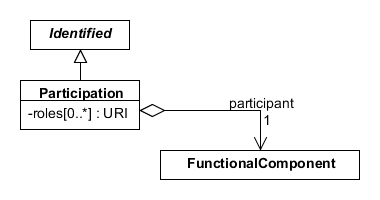
\includegraphics[scale=0.6]{uml/participation}
\caption[]{Diagram of the \sbol{Participation} class and its associated properties.}
\label{uml:participation}
\end{center}
\end{figure}

\subparagraph{The \sbolheading{role} property}\label{sec:role:P}

A \sbol{Participation} is REQUIRED to have one or more \sbolmult{role:I}{role} properties, each of type \sbol{URI} that describes the behavior of a \sbol{Participation} (and by extension its referenced \sbol{Feature}) in the context of its parent \sbol{Interaction}.

Each \sbolmult{role:P}{role} property MUST identify terms from appropriate ontologies. It is RECOMMENDED that exactly one \sbol{URI} specified by a \sbolmult{role:P}{role} property refer to a term from the participant role branch of the SBO. \ref{tbl:participant_roles} provides a partial list of possible SBO terms for the \sbolmult{role:P}{role} properties and their corresponding \sbol{URI}s.

\begin{table}[ht]
  \begin{edtable}{tabular}{lll}
    \toprule
    \textbf{Participation Role} & \textbf{URI for SBO Term} & \textbf{Interaction Types}\\
    \midrule
    Inhibitor  & \url{http://identifiers.org/biomodels.sbo/SBO:0000020} & Inhibition\\
    Inhibited  & \url{http://identifiers.org/biomodels.sbo/SBO:0000642} & Inhibition\\
    Stimulator & \url{http://identifiers.org/biomodels.sbo/SBO:0000459}  & Stimulation\\
    Stimulated & \url{http://identifiers.org/biomodels.sbo/SBO:0000643}  & Stimulation\\
     Reactant & \url{http://identifiers.org/biomodels.sbo/SBO:0000010}  & Non-Covalent Binding, Degradation \\
     & & Biochemical Reaction \\
    Product & \url{http://identifiers.org/biomodels.sbo/SBO:0000011}  & Non-Covalent Binding, \\
    & & Genetic Production, Biochemical Reaction\\
    Promoter  & \url{http://identifiers.org/biomodels.sbo/SBO:0000598} & Inhibition, Stimulation, Genetic Production\\
    Modifier  & \url{http://identifiers.org/biomodels.sbo/SBO:0000019} & Biochemical Reaction, Control\\
    Modified  & \url{http://identifiers.org/biomodels.sbo/SBO:0000644} & Biochemical Reaction, Control\\
    Template  & \url{http://identifiers.org/biomodels.sbo/SBO:0000645} & Genetic Production\\
%    Ligand & \url{http://identifiers.org/biomodels.sbo/SBO:0000280}\\
%    Non-Covalent Complex & \url{http://identifiers.org/biomodels.sbo/SBO:0000253}\\
    \bottomrule
  \end{edtable}
  \caption{Partial list of SBO terms to specify the \sbolmult{role:P}{role} properties of a \sbol{Participation}.}
  \label{tbl:participant_roles}
\end{table}

If a \sbol{Participation} is well described by one of the terms from \ref{tbl:participant_roles}, then a \sbolmult{role:P}{role} property MUST refer to the \sbol{URI} that identifies this term.  Also, if a \sbol{Participation} belongs to an \sbol{Interaction} that has a type listed in \ref{tbl:interaction_types}, then the \sbol{Participation} SHOULD have a role that is cross-listed with this type in \ref{tbl:participant_roles}.  Lastly, if there are multiple \sbolmult{role:P}{role} properties for a \sbol{Participation}, then they MUST identify non-conflicting terms. For example, the SBO terms ``stimulator'' and ``inhibitor'' would conflict.

\subparagraph{The \sbolheading{participant} property}\label{sec:participant}

The \sbol{participant} property MUST specify precisely one \sbol{Feature} object that plays the designated role in its parent \sbol{Interaction} object.

